\begin{surferPage}[Бартова површ]{Бартова површ шестог степена}
    Ову површ шестог степена је конструисао Волф Барт 1996. године. Ова површ има укупно 65 сингуларитета.
%    (wenn man die $15$ im Bild nicht sichtbaren, ``unendlich fernen'', mitzählt)%
   Ово је максималан број сингуларитета за било коју површ шестог степена, што су показали непосредно после Бартове конструкције Џафе и Руберман – значи, Бартов светски рекорд је необорив!


    Бартова конструкција је била велико изненађење јер се дуго сматрало да површи шестог степена могу да имају само 64 сингуларитета.

   Упечатљива особина ове конструкције је њена симетрија икосаедра; на слици је икосаедар и његове равни симетрија:  
%    Die Abb.\ zeigt diesen platonischen Körper und seine Symmetrie - Ebenen: 
%    und diese Ebenen gemeinsam mit der Barth Sextik in einem Bild.     
    % 
  \begin{center}
      \vspace*{-0.1cm}
      \begin{tabular}{@{}c@{\ \ }c@{\,}c@{}}
        \begin{tabular}{@{}c}
          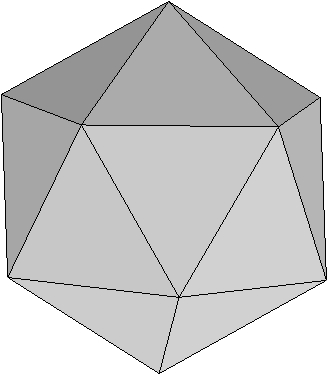
\includegraphics[width=1.4cm]{icosah}
        \end{tabular}
        &
        \begin{tabular}{@{}c}
          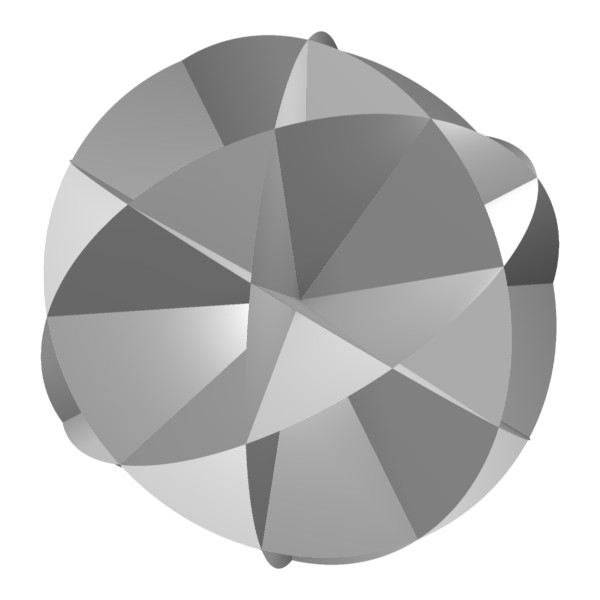
\includegraphics[width=1.4cm]{barth_sextic_planes}
        \end{tabular}
        &
        \begin{tabular}{c@{}}
          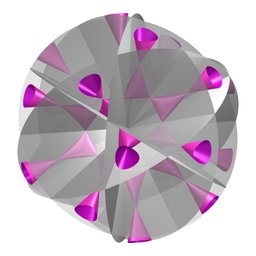
\includegraphics[width=1.4cm]{barth_sextic_and_planes}
        \end{tabular}
      \end{tabular}
    \end{center}
    \vspace*{-0.1cm}

    Бартова површ  задовољава једначину 
    $P_6 - \alpha K^2=0,$ где $P_6$
    означава 6 равни симетрија, $K=x^2+y^2+z^2-1$ је јединична сфера и  
    $\alpha=\frac{1}{4}(2+\sqrt{5})$.
\end{surferPage}
